\begin{enunciado}
 En el ejercicio 1.19 de la p\'agina 28, pruebe la bondad de ajuste
 entre las frecuencias de clase que se observan
 y las frecuencias esperadas correspondientes de una distribuci\'on normal
 con $\mu = 1.8$ y $\sigma = 0.4$.
 Utilice un nivel de significancia de $0.01$.
\end{enunciado}

\begin{solucion}
 La resoluci\'on se har\'a usando ambas pruebas vistas en el libro:
 la prueba de bondad de ajuste $\chi^2$ y la prueba de Geary.
 \begin{datos}
  Usando los datos del ejercicio 1.19, incluyendo el diagrama de tallo y hoja, 
  se tiene lo siguiente:
  \begin{itemize}
   \item Tama\~no de la muestra: $n=30$.
   \item Media muestral: $\bar{x} = \frac{829}{300} = 2.79\bar{6}$.
   \item Varianza muestral:
   $s^2 = \frac{431\,609}{87\,000} \approx 4.96102$
   \item Frecuencia observada individualmente:
   \begin{center}
    \begin{tabular}{cccccc}
     $2.0$ & $3.0$ & $0.3$ & $3.3$ & $1.3$ & $0.4$ \\
     $0.2$ & $6.0$ & $5.5$ & $6.5$ & $0.2$ & $2.3$ \\
     $1.5$ & $4.0$ & $5.9$ & $1.8$ & $4.7$ & $0.7$ \\
     $4.5$ & $0.3$ & $1.5$ & $0.5$ & $2.5$ & $5.0$ \\
     $1.0$ & $6.0$ & $5.6$ & $6.0$ & $1.2$ & $0.2$ 
    \end{tabular}
   \end{center}
   las cuales se pueden agrupar en las $7$ clases que hicieron
   en el diagrama de tallo y hoja del ejercicio al que se hace referencia, 
   lo cual se muestra en la siguiente tabla:
   \begin{center}
    \begin{tabular}{cc}
     \hline 
     \textbf{L\'{\i}mites de clase} & $o_i$ \\
     \hline 
     $-0.05 - 0.95$ &  $8$ \\
     $0.95 - 1.95$ & $6$ \\
     $1.95 - 2.95$ & $3$ \\
     $2.95 - 3.95$ & $2$ \\
     $3.95 - 4.95$ & $3$ \\
     $4.95 - 5.95$ & $4$ \\
     $5.95 - 6.95$ & $4$ \\
     \hline 
    \end{tabular}
   \end{center}
   \item Probabilidades esperadas: usando la tabla A.3,
   se encuentra las \'areas bajo la curva para cada clase como sigue:
   \begin{center}
    \begin{tabular}{cccc}
     \hline 
     \multicolumn{3}{c}{\textbf{L\'{\i}mites de clase}} & $p_i$ \\
     \hline 
     $-0.05$ & $-$ & $0.95$ &
     $P\left( Z<\frac{0.95 - 1.8}{0.4}\right) \approx P(Z<-2.125)\approx 0.0168$ \\
     $0.95$ & $-$ & $1.95$ &
     $P\left( \frac{0.95 - 1.8}{0.4} < Z < \frac{1.95 - 1.8}{0.4} \right)
     \approx P(Z < 0.375) - P(Z < -2.125)$ \\
     & & & $\approx 0.6461 - 0.0168 = 0.6293$ \\
     $1.95$ & $-$ & $2.95$ &
     $P\left( \frac{1.95 - 1.8}{0.4} < Z < \frac{2.95 - 1.8}{0.4} \right)
     \approx P(Z < 2.875) - P(Z < 0.375)$ \\
     & & & $\approx 0.998 - 0.6461 = 0.3519$ \\
     $2.95$ & $-$ & $3.95$ &
     $P\left( \frac{2.95 - 1.8}{0.4} < Z < \frac{3.95 - 1.8}{0.4} \right)
     \approx P(Z < 5.375) - P(Z < 2.875)$ \\
     & & & $\approx 1 - 0.998 = 0.002$ \\
     $3.95$ & $-$ & $4.95$ &
     $P\left( \frac{3.95 - 1.8}{0.4} < Z < \frac{4.95 - 1.8}{0.4} \right)
     \approx P(Z < 7.875) - P(Z < 5.375)$ \\
     & & & $\approx 1 - 1 = 0$ \\
     $4.95$ & $-$ & $5.95$ &
     $P\left( \frac{4.95 - 1.8}{0.4} < Z < \frac{5.95 - 1.8}{0.4} \right)
     \approx P(Z < 10.375) - P(Z < 7.875)$ \\
     & & & $\approx 1 - 1 = 0$ \\
     $5.95$ & $-$ & $6.95$ &
     $P\left( Z > \frac{5.95 - 1.8}{0.4} \right) \approx 1 - P(Z < 10.375)$ \\
     & & & $\approx 1 - 1 = 0$ \\
     \hline
    \end{tabular}
   \end{center}
   \item Frecuencias esperadas, determinado por clase
   y considerando el redondeo a un decimal: $E = \left\{
   \left.e_i=n\cdot p_i\,\right|\,\forall i\in\mathbb{N}\cap[1,7] \right\}
   = \{ e_1 = 30\times 0.0168 = 0.5, e_2 = 30 \times 0.6292 = 18.9,
   e_3 = 30 \times 0.3519 = 10.6, e_4 = 30 \times 0.0002 = 0,
   e_5 = 30 \times 0 = 0, e_6 = 30 \times 0 = 0,
   e_7 = 30 \times 0 = 0 \}$
  \end{itemize}
  Dado que las pruebas de bondad por m\'etodo de $\chi^2$ no son confiables
  cuando la frecuencia esperada de una celda es menor a $5$,
  se agrupar\'an los datos, como sigue:
  \begin{itemize}
   \item Frecuencias observadas, probabilidades esperadas y frecuencias
   esperadas por clase, se muestran a continuaci\'on en la siguiente tabla:
   \begin{center}
    \begin{tabular}{ccccccc}
     \hline
     \textbf{L\'{\i}mites de clase} & $o_i$ & & $p_i$ & & $e_i$ & \\
     \hline 
     $-0.05 - 0.95$ &  $8$ &
     \multirow{2}{*}{\hspace{-0.7cm} $\left.
     \begin{matrix} \phantom{0} \\ \phantom{0} \end{matrix}
     \right\} 14$}
     & $0.0168$ &
     \multirow{2}{*}{\hspace{-0.5cm}$\left.
     \begin{matrix} \phantom{0} \\ \phantom{0} \end{matrix}
     \right\} 0.646$}
     & $0.5$ &
     \multirow{2}{*}{\hspace{-0.7cm} $\left.
     \begin{matrix} \phantom{0} \\ \phantom{0} \end{matrix}
     \right\} 19.4$} \\
     $0.95 - 1.95$ & $6$ &\hspace{-0.7cm}& $0.6292$ &\hspace{-0.5cm}& $18.9$  \\
     $1.95 - 2.95$ & $3$ &
     \multirow{5}{*}{\hspace{-0.7cm} $\left.
     \begin{matrix} \phantom{0} \\ \phantom{0} \\ \phantom{0}
     \\\phantom{0} \\ \phantom{0} \end{matrix}
     \right\} 16$}
     & $0.3519$ &
     \multirow{5}{*}{\hspace{-0.5cm}$\left.
     \begin{matrix} \phantom{0} \\ \phantom{0} \\ \phantom{0}
     \\\phantom{0} \\ \phantom{0} \end{matrix}
     \right\} 0.3521$}
     & $10.6$ &
     \multirow{5}{*}{\hspace{-0.7cm} $\left.
     \begin{matrix} \phantom{0} \\ \phantom{0} \\ \phantom{0}
     \\\phantom{0} \\ \phantom{0} \end{matrix}
     \right\} 10.6$} \\     
     $2.95 - 3.95$ & $2$ &\hspace{-0.7cm}& $0.0002$ &\hspace{-0.5cm}& $0$ \\
     $3.95 - 4.95$ & $3$ &\hspace{-0.7cm}& $0$ &\hspace{-0.5cm}& $0$ \\
     $4.95 - 5.95$ & $4$ &\hspace{-0.7cm}& $0$ &\hspace{-0.5cm}& $0$ \\
     $5.95 - 6.95$ & $4$ &\hspace{-0.7cm}& $0$ &\hspace{-0.5cm}& $0$ \\
     \hline 
    \end{tabular}
   \end{center}
   \item Celdas totales del experimento: $k=2$.
   \item Grados de libertad de la prueba $\chi^2$: $v= k-1 = 1$.
  \end{itemize}
 \end{datos}
 
 \begin{hipotesis}
  Prueba de bondad de ajuste para probar $H_0:$
  que la variable aleatoria $X$, de los a\~nos de vida de las bombas
  de combustible de cierto tipo, sigue una distribuci\'on normal
  con media $\mu=1.8$ y desviaci\'on est\'andar $\sigma = 0.4$,
  contra la alternativa $H_1$ de que no es as\'{\i}.
 \end{hipotesis}

 \begin{significancia}
  $\alpha = 0.01$.
 \end{significancia}

 \begin{region}
  De la tabla A.5, se tiene el valor cr\'{\i}tico
  $\chi^2_{\alpha,v} = \chi^2_{0.01,1} \approx 6.635$,
  por lo que la regi\'on de rechazo est\'a dado
  para $\chi^2 > 6.635$, donde
  $\chi^2 = \sum_{i=1}^{k} \frac{\left( o_i - e_i \right)^2}{e_i}$.
  O bien, de la tabla A.3, se tiene el valor cr\'{\i}tico
  $Z_{\alpha/2} = Z_{0.005} \approx 2.575$,
  por lo que la regi\'on de rechazo tambi\'en est\'a dado
  para $Z < -2.575$ o $Z > 2.575$,
  donde $Z = \frac{U - 1}{0.2661/\sqrt{n}}$ y, a su vez,
  $U = \frac{\sqrt{\pi/2} \sum_{i=1}^{n} \left| X_i - \overline{X} \right|/n}{
  \sqrt{\sum_{i=1}^n \left( X_i - \overline{X} \right)^2/n}}$
 \end{region}

 \begin{estadistico}
  Para la prueba de $\chi^2$, el estad\'{\i}stico est\'a dado por:
  \begin{eqnarray*}
   \chi^2 & = & \sum_{i=1}^{k} \frac{\left( o_i - e_i \right)^2}{e_i} \\
   & \approx & \frac{(14-19.4)^2}{19.4} + \frac{(16-10.6)^2}{10.6} \\
   & = & \frac{(-5.4)^2}{19.4} + \frac{5.4^2}{10.6}
   = \frac{29.16(53) + 29.16(97)}{1\,028.2}
   = \frac{4\,374}{1\,028.2} \\
   & = & \frac{21\,870}{5\,141} \approx 4.254
  \end{eqnarray*}
  Mientras que, para la prueba de Geary, el c\'alculo del estad\'{\i}stico
  se realiza como sigue, realizando previamente algunos c\'alculos:
  \par 
  Primero se requieren los valores de $x_i - \bar{x}$, los cuales se
  han calculado en el proceso de obtener la desviaci\'on est\'andar
  durante la soluci\'on del problema 1.19, luego entonces, se tiene que:
  \begin{eqnarray*}
   \sum_{i=1}^{60} \left| x_i - \overline{x} \right| & = &
   \frac{1}{30}\left( |-23.9| + |6.1| + |-74.9| + |15.1| + |-44.9| + |-71.9| +
   |-77.9| + \right. \\
   & & \phantom{\frac{1}{60}(}  |96.1| + |81.1| + |111.1| + |-77.9| + |-14.9| +
   |-38.9| + |36.1| + |93.1| + \\
   & & \phantom{\frac{1}{60}(} |-29.9| + |57.1| + |-62.9| + |51.1| + |-74.9| +
   |-38.9| + |68.9| + \\
   & & \phantom{\frac{1}{60}} \left. |-8.9| + |66.1| + |-53.9| + |96.1| + 
   |84.1| + |96.1| + |-47.9| + |-77.9| \right) \\
   & = & \frac{1\,778.6}{30} = \frac{8\,893}{150} = 59.28\bar{6}
  \end{eqnarray*}
  y
  \begin{equation*}
   \sum_{i=1}^{60} \left( x_i - \overline{x} \right)^2 = s^2\times 29 =
   \frac{431\,609}{\cancelto{3\,000}{87\,000}}\hspace{0.7cm}\times \cancel{29}
   = \frac{431\,609}{3\,000} = 143.869\bar{6}
  \end{equation*}
  Luego entonces
  \begin{eqnarray*}
   U & = & \frac{
   \displaystyle{\sqrt{\pi/2}
   \frac{\sum_{i=1}^n \left| X_i - \overline{X} \right|}{n}}
   }{
   \displaystyle{\sqrt{
   \frac{\sum_{i =1}^n \left( X_i - \overline{X} \right)^2}{n}}}
   } 
   = \frac{\displaystyle{\sqrt{\pi/2} \frac{8\,893}{4\,500}}}{
   \displaystyle{\sqrt{ \frac{431\,609}{90\,000} }}}
   = \frac{\displaystyle{\sqrt{\pi} \frac{8\,893}{\cancelto{15}{4\,500}}}}{
   \displaystyle{
   \frac{\sqrt{2\times 431\,609}}{\cancel{300}} 
   }}
   = \frac{\sqrt{863\,218\pi} 8\,893}{863\,218 \times 15} \\
   & = & \frac{\sqrt{863\,218\pi} 8\,893}{12\,948\,270}
   \approx 1.13102
  \end{eqnarray*}
  Por lo que el estad\'{\i}stico $Z$ para la prueba de Geary es:
  \begin{eqnarray*}
   Z & = & \frac{U - 1}{0.2661/\sqrt{n}} = 
   \frac{\displaystyle{\frac{\sqrt{863\,218\pi} 8\,893}{12\,948\,270} - 1}
   }{\displaystyle{\frac{0.2661}{\sqrt{30}}}}
   = \frac{\displaystyle{
   \frac{\sqrt{863\,218\pi} 8\,893 - 12\,948\,270}{12\,948\,270}}}{
   \displaystyle{\frac{2\,661}{10\,000\cdot \sqrt{30}}}} \\
   & = & \frac{\cancelto{1\,000}{10\,000}\,\,\,\sqrt{30} \cdot
   \left(\sqrt{863\,218\pi} 8\,893 - 12\,948\,270\right)}{
   2\,661\cdot \cancelto{1\,294\,827}{12\,948\,270}} \\
   & = & \frac{1\,000\sqrt{30} \cdot
   \left(\sqrt{863\,218\pi} 8\,893 - 12\,948\,270\right)}{
   3\,445\,534\,647} \approx 2.6969 \\
  \end{eqnarray*}
 \end{estadistico}

 \begin{decision}
  Se presenta una discrepancia al comparar las pruebas de bondad de $\chi^2$
  y de Geary.
  En la literatura se sugiere que, si existe discrepancia entre dos pruebas,
  se debe tomar una decisi\'on conservadora, es decir,
  se rechaza $H_0$ a favor de $H_1$.
 \end{decision}

 \begin{conclusion}
  Se obtiene evidencia suficiente, por la prueba de Geary, para afirmar
  que los a\~nos de vida de las bombas de combustible similares analizados
  no sigue una distribuci\'on normal con media $\mu = 1.8$
  y desviaci\'on est\'andar $\sigma = 0.4$.
 \end{conclusion}

 Finalmente, usando el archivo anexo
 \texttt{P17\_Prueba\_de\_normalidad\_01.r},
 que a su vez requiere los datos del archivo \texttt{BD25\_Problema\_089.csv},
 con los siguientes cambios:
 \begin{verbatim}
> datos<-read.csv("DB25_Problema_089.csv",sep=";",encoding="UTF-8")
> varInteres<-"Duración.años"
> media<-1.8
> desv.est<-0.4
> clases<-c(-0.05,0.95,1.95,2.95,3.95,4.95,5.95,6.95)
> graficaHist<-TRUE
 \end{verbatim}
 \vspace{-0.5cm}
 el programa de R lanza el siguiente resultado:
 \begin{verbatim}
        nombres  n X de chi2 param chi2 Valor-p chi2 Z de Geary Valor-p Geary
1 Duración.años 30  4.227889          1   0.03976487   2.696906   0.006998705
   D de K-S Valor-p K-S D de K-S Lilliefors Valor-p K-S Lilliefors W de Shapiro
1 0.4599408 3.64055e-05            0.153104             0.07061746    0.8789531
  Valor-p Shapiro
1     0.002667603
 \end{verbatim}
 \vspace{-0.5cm}
 que incluye la siguiente figura:
 \begin{center}
  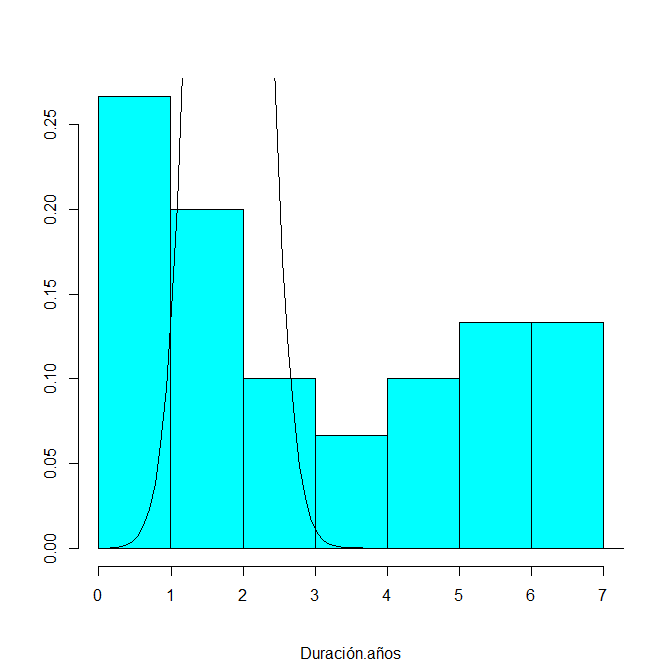
\includegraphics[scale=0.35]{Problema_89.png}
 \end{center}
 Lo cual coincide con los resultado obtenidos.
 Se hace notar que los resultados usando las pruebas K-S y Lilliefors
 requieren de tama\~nos grandes de muestra, mayores a 100,
 por lo que no se toma en cuenta.
 Por otro lado, la prueba de Shapiro, aunque da buenos resultados
 en pruebas peque\~nas como esta, no se est\'a considerando los par\'ametros
 supuestos, como es el caso de la prueba Geary.
 En este caso, parecer\'{\i}a que la \'unica que tiene validez suficiente
 es la prueba $\chi^2$, pero,
 tomando en cuenta de que los par\'ametros estimados para la media y varianza
 son las m\'as probables en las pruebas de Shapiro-Wilk y de Geary,
 entonces se pueden tomar en cuenta como pruebas
 generales para saber si se est\'a distribuyendo a la normal m\'as probable,
 lo cual todo indica que no,
 mientras que la prueba $\chi^2$ de Pearson arroja un valor $P$ muy bajo.
 Entonces, por la direcci\'on a la que se est\'a llevando estas observaciones,
 es razonable llegar a que ciertamente es poco probable
 que la poblaci\'on de la que viene la muestra se distribuya normalmente.
 Finalmente, existe una diferencia entre el valor del estad\'{\i}stico
 $\chi^2$ que se muestra en las soluciones del libro
 con el que se muestra en esta soluci\'on.
 Esto se debe a c\'omo se consideraron las clases,
 de una forma m\'as conservadora,
 y se puede revisar que coincide mejor el resultado
 si se modifica la siguiente l\'{\i}nea en el programa:
 \begin{verbatim}
> clases<-c(0,1,2,3,4,5,6,7)
 \end{verbatim}
 \vspace{-0.5cm}
 lo cual arroja como valor del estad\'{\i}stico el n\'umero
 \texttt{5.154801};
 tambi\'en se muestra una decisi\'on distinta en la soluci\'on del libro,
 lo cual se debe a que \'unicamente se considera la prueba $\chi^2$
 en el libro, lo cual puede ser insuficiente
 al comparar con otras pruebas como se hizo en esta soluci\'on.
 Que es a lo que se quer\'{\i}a llegar.${}_{\blacksquare}$
\end{solucion}
